
%%%%%%%%%%%%%%%%
%%%%%%%%%%%%%%%%

\section{An improved DEC analysis}

In this section, we'll focus on techniques that allow permit more realistic biogeographic analyses.
Topics include applying range size constraints, area connectivity, stratified/epoch models, function-valued dispersal rates, and incorporating uncertainty in paleogeographic event time estimates.

Start by creating our filename variables

\begin{snugshade}
\begin{lstlisting}
range_fn = "data/n4/silversword.n4.range.nex"
phy_fn   = "data/n4/silversword.tre"
out_fn   = "output/complex"
geo_fn   = "data/n4/hawaii.n4"
times_fn = geo_fn + ".times.txt"
dist_fn  = geo_fn + ".distances.txt"
\end{lstlisting}
\end{snugshade}

Create some helper analysis variables

\begin{snugshade}
\begin{lstlisting}
mvi = 1
mni = 1
n_gen = 1e3
\end{lstlisting}
\end{snugshade}


Read in the presence-absence range characters and record the number of areas in the dataset

\begin{snugshade}
\begin{lstlisting}
dat_range_01 = readDiscreteCharacterData(range_fn)
n_areas <- dat_range_01.nchar()
\end{lstlisting}
\end{snugshade}

Often, biogeographers wish to limit to the maximum allowable range size.
This prohibits widespread species ranges and to reduce the total number of range states in the analysis, thus benefitting computational efficiency.
Suppose we disallowed ranges from including more than two areas.
The total number of ranges equals $\sum_{k=0}^m {{n}\choose{k}}$ where $n$ is the total number of areas, $m$ is the maximum number of permissible areas, and ${{n}\choose{k}}$ is the number of ways to sample $k$ unordered areas from a pool of $n$ areas.

\begin{snugshade}
\begin{lstlisting}
max_areas <- 2
n_states <- 0
for (k in 0:max_areas) n_states += choose(n_areas, k)
\end{lstlisting}
\end{snugshade}

Then format the dataset for the reduced state space

\begin{snugshade}
\begin{lstlisting}
dat_range_n = formatDiscreteCharacterData(dat_range_01, "DEC", n_states)
\end{lstlisting}
\end{snugshade}

Our state space now includes only 11 states ($\emptyset$, K, O, M, H, KO, KM, OM, KH, OH, MH).

% read in some geography data
Next, we'll set up the paleogeographic model.
Read in the list of minimum and maximum ages of island formation

\begin{snugshade}
\begin{lstlisting}
time_bounds <- readDataDelimitedFile(file=times_fn, delimiter=" ")
n_epochs <- time_bounds.size()
\end{lstlisting}
\end{snugshade}

Read in a vector of matrices that describe the connectivity between areas over time.
Note, there is one connectivity matrix per epoch, ordered from oldest to youngest.

\begin{snugshade}
\begin{lstlisting}
for (i in 1:n_epochs) {
    connectivity[i] <- readDataDelimitedFile(file=geo_fn+"."+i+".txt", delimiter=" ")
}
\end{lstlisting}
\end{snugshade}

Read in the matrix of distances between all pairs of areas (km). For simplicity, we will assume that distances remain constant over time, even though they certainly vary.

\begin{snugshade}
\begin{lstlisting}
distances <- readDataDelimitedFile(file=dist_fn, delimiter=" ")
\end{lstlisting}
\end{snugshade}


% distances between areas

Dispersal rates might make use of some extrinsic information, such as geographical distances between areas \citep{macarthur67, webb12}.
We model this as $d_{ij} = a e ^ {-b g_{ij}}$ where $g_{ij}$ is the geographical distance between areas $i$ and $j$ and $a$ and $b$ are parameters that scale distance on linear and exponential scales, respectively. Note that all dispersal rates equal $a$ when $b=0$.

\begin{snugshade}
\begin{lstlisting}
a ~ dnGamma(2,2)
moves[mvi++] = mvScale(a)
b ~ dnUniform(-5,5)
b.setValue(0)
moves[mvi++] = mvSlide(b, delta=0.1)
\end{lstlisting}
\end{snugshade}

Now we can assign rates that are functions of distance between all pairs of areas

%dr[i][j][k] := (a * exp( -b * distances[j][k] ))
\begin{snugshade}
\begin{lstlisting}
for (i in 1:n_epochs) {
    for (j in 1:n_areas) {
        for (k in 1:n_areas) {
            dr[i][j][k] <- abs(0)
            if (connectivity[i][j][k] > 0) {
                dr[i][j][k] := a * exp( -b * distances[j][k] )
            }
        }
    }
}
\end{lstlisting}
\end{snugshade}


% extirpation penalized ranges
% ... they can exist, but not persist

It is unlikely that widespread ranges persist across disjunct areas for long periods of time.
Extirpation is more likely to occur in fragmented ranges than well-connected ranges, where peripheral populations are continuously reinforced from the center.

\begin{snugshade}
\begin{lstlisting}
e ~ dnExp(1)
moves[mvi++] = mvScale(e)

for (i in 1:n_epochs) {
    for (j in 1:n_areas) {
        for (k in 1:n_areas) {
            er[i][j][k] <- abs(0)
            if (j == k) {
                er[i][j][k] := e
            }
        }
    }
}

\end{lstlisting}
\end{snugshade}


% uncertainty in paleogeographic events

Treat epoch times as random variables. The present is always the present.
\begin{snugshade}
\begin{lstlisting}
for (i in 1:n_epochs) {
    time_max[i] <- time_bounds[i][1]
    time_min[i] <- time_bounds[i][2]
    if (i != n_epochs) {
        epoch_times[i] ~ dnUniform(time_min[i], time_max[i])
        moves[mvi++] = mvSlide(epoch_times[i], delta=0.5)
    } else {
        epoch_times[i] <- 0.0
    }
}
\end{lstlisting}
\end{snugshade}


% epoch model for anagenetic change

Build a rate matrix for each time interval
\begin{snugshade}
\begin{lstlisting}
for (i in 1:n_epochs) {
    Q_DEC[i] := fnDECRateMatrix(dispersalRates=connectivity[i],
                            extirpationRates=er,
                            maxRangeSize=max_areas)
}
\end{lstlisting}
\end{snugshade}


Create the epoch rate generator object
\begin{snugshade}
\begin{lstlisting}
Q_DEC_epoch := fnDECCladoProbs(Q=Q_DEC, times=epoch_times, rates=rep(1,n_epochs))
\end{lstlisting}
\end{snugshade}

% clado event probs

Here, we treat the probability of different types of cladogenetic events as a random variable to be estimate.

\begin{snugshade}
\begin{lstlisting}
clado_event_types <- [ "s", "a" ]
clado_type_probs ~ dnDirichlet( [1,1] )
moves[++mi] = mvSimplexElementScale(clado_type_probs, alpha=10)
P_clado := fnDECCladoProbs(eventProbs=clado_type_probs,
                           eventTypes=clado_event_types,
                           numCharacters=n_areas,
                           maxRangeSize=max_areas)
\end{lstlisting}
\end{snugshade}

For this dataset, we assume cladogenetic probabilities are constant with respect to geological time.


\begin{snugshade}
\begin{lstlisting}
rate_bg <- 1
\end{lstlisting}
\end{snugshade}


\begin{snugshade}
\begin{lstlisting}
rf_DEC <- rep(0, n_states)
rf_DEC[2] <- 1
rf_DEC <- simplex(rf_DEC)
\end{lstlisting}
\end{snugshade}


Create the phylogenetic model
\begin{snugshade}
\begin{lstlisting}
ctmc_bg ~ dnCTMCClado(tree=phy,
                      Q=Q_DEC_epoch,
                      cladoProbs=P_DEC,
                      branchRates=rate_bg,
                      rootFrequencies=rf_DEC,
                      type="NaturalNumbers",
                      nSites=1)
                  
\end{lstlisting}
\end{snugshade}


Attach the dataset
\begin{snugshade}
\begin{lstlisting}
ctmc_bg.clamp(dat_range_n)
\end{lstlisting}
\end{snugshade}


And the rest we've done before...
\begin{snugshade}
\begin{lstlisting}
# make the model
mdl = model(m)

# make the monitors
mn[1] = mnScreen(dispersal_rate, distance_scale, extirpation_rate, printgen=1000)
mn[2] = mnModel(file=out_fn+".params.txt", printgen=100)
mn[3] = mnJointConditionalAncestralState(tree=psi, ctmc=m, filename=out_fn+".states.txt", type="NaturalNumbers", printgen=100, withTips=true, withStartStates=true)

# make and run MCMC
ch = mcmc(mv,mn,mdl)
ch.burnin(1000, 10)
ch.run(10000)
\end{lstlisting}
\end{snugshade}

The ancestral state estimates look much more realistic, given what we know about when the islands were formed and the speciation times.

\begin{figure}[!ht]
\centering
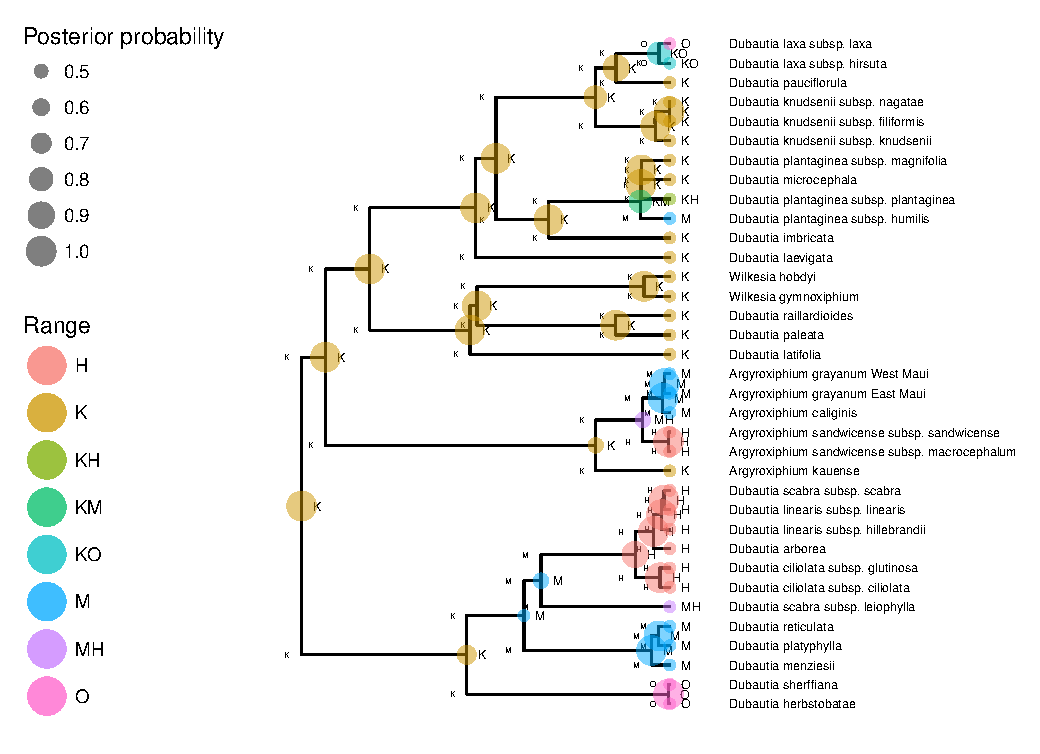
\includegraphics[width=0.7\textwidth]{figures/fig_epoch_RevGadgets_ase.pdf}
\caption{Tree with ancestral state estimates. Nodes are annotated with ancestral states before and after cladogenetic events. Most probable states are shown. Colors of markers indicate the range state. Sizes of markers indicate the posterior probability of that state. }
\end{figure}

[ Look at posterior estimates for distance. ]

\newpage
